\chapter{基于深度学习的多实例点云配准}
现有的工作主要集中在单对单的物体或场景同级别的点云配准,该方向上的工作已经十分成熟,传统的ICP配准方法\cite{barath2021progressive, li2020evaluation, shi2020improved}和深度学习方法\cite{qin2022geometric,barath2019progressive,barath2021progressive}都能达到很好的效果。但是,目前的工作对于物体对场景中多个物体的不同级别的多个配准表现仍然有待提升。本文主要构建了一种基于对应聚类方法的多实例点云配准模型和一种基于对比学习的多实例点云配准模型,将在本章展开讨论。
\section{问题陈述}

在多实例点云配准问题中,源点云$\boldsymbol{X}$提供了一个3D模型的实例,目标点云$\boldsymbol{Y}$包含了这个模型的$K$个实例,其中这些实例是一组点的集合,这些点可能只采样了3D模型的一部分。如果本文将第$k^{th}$个实例写为$\boldsymbol{Y}_k$,那么目标点云$\boldsymbol{Y}$可以分解为$
%\begin{equation}
\boldsymbol{Y} = \boldsymbol{Y}_0 \cup \boldsymbol{Y}_1 \cup \ldots \boldsymbol{Y}_k \ldots \cup \boldsymbol{Y}_K$。
%\end{equation}
这里本文使用$\boldsymbol{Y}_0$表示点云中不属于任何实例的部分。
多实例3D配准的目标是找到刚性变换$(\boldsymbol{R}_k, \boldsymbol{t}_k)$,将源实例$\boldsymbol{X}$对准到每个目标实例$\boldsymbol{Y}_k$。
如果本文设法获得源实例与每个目标实例$\boldsymbol{X} \leftrightarrow \boldsymbol{Y}_k$之间的点对关系,那么通过最小化对齐误差之和(\ref{eq:solve_rigid_transform}) \cite{levinson2020analysis},可以从点对关系集合$\boldsymbol{X}\leftrightarrow \boldsymbol{Y}_k$中求解目标点云中第$k^{th}$个实例的位姿$(\boldsymbol{R}_k, \boldsymbol{t}_k)$:
\begin{equation}
\underset{\boldsymbol{R}_k,\boldsymbol{t}_k}{\min}\sum_i{\parallel}\boldsymbol{y}_{ki}-(\boldsymbol{R}_k\boldsymbol{x}_i+\boldsymbol{t}_k)\parallel ^2.
\label{eq:solve_rigid_transform}
\end{equation}
考虑到本文已经获得了源点云和目标点云之间的一组点对关系$\mathcal{C}$。多实例配准任务的关键是将这些点对关系分类为与不同实例相关的独立集合,即:
\begin{equation}
\mathcal{C} = \mathcal{C}_0 \cup \mathcal{C}_1\cdots \cup \mathcal{C}_K.
\end{equation}
这里,$\mathcal{C}_0$用来表示异常值集合。如本文所见,多实例配准不仅需要剔除异常值点对关系,还需要解决来自不同实例的点对关系的歧义。这个任务并不容易,因为所有实例看起来都一样,而且通常存在大量的异常值点对关系。

\section{高效对应聚类的多实例点云配准 ECC}

\subsection{结构模型}
本文提出的方法的概述如图 \ref{fig:multicluster} 所示,从输入点对关系构建距离不变性矩阵,用于将点对关系聚类为不同的簇(\textbf{聚类}),并进行优化(\textbf{簇优化})。最后,从每个点对关系簇中估计与每个实例相关的刚体变换(\textbf{变换})。为了处理大量的点对关系,采用两个附加过程(\textbf{下采样}和\textbf{上采样})。详细内容将在接下来的章节中介绍。

\begin{figure*}[ht]
    \centering
    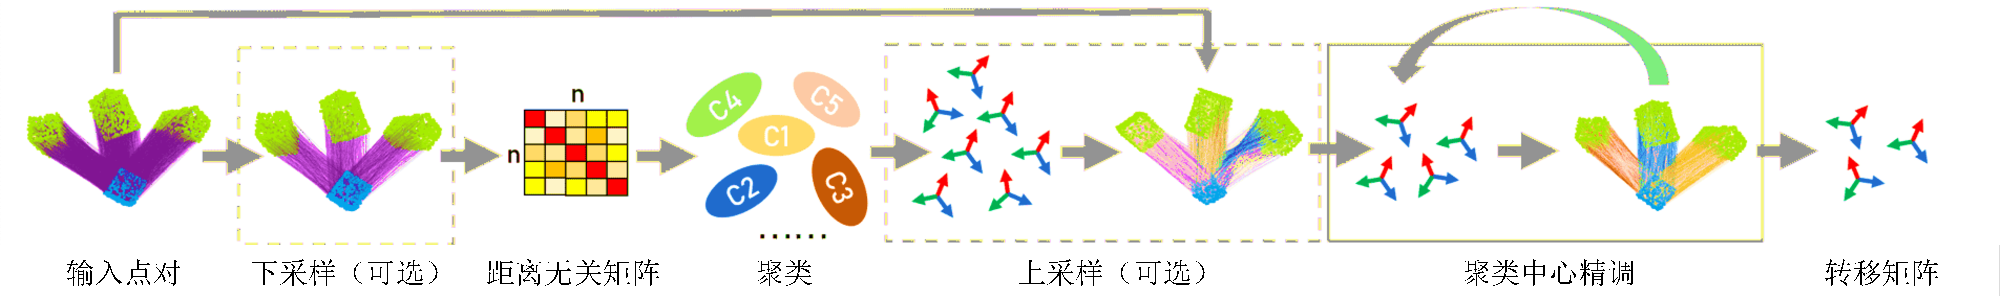
\includegraphics[width=1\textwidth]{images/multi-cluster.pdf}
    \caption{多实例点云配准方法的流程。}
    \label{fig:multicluster}
    \vspace{-0.6in}
\end{figure*}

\subsection{基于不变型矩阵的聚类}
\label{subsec:Distance-Consistency-Graph}
距离不变性特性在3D配准领域已经被研究多年\cite{yang2020teaser, shi2021robin,leordeanu2005spectral},该特性描述了在刚性变换之后两点之间的距离保持不变。具体来说,如果 $c_i :\boldsymbol{x}_i \leftrightarrow \boldsymbol{y}_i$ 和 $c_j : \boldsymbol{x}_j \leftrightarrow \boldsymbol{y}_j$ 是两个真实的点对关系,那么它们应该满足
%
\begin{equation}
G_{ij}=|d_{ij} - d'_{ij} | < \delta
\label{eq:abs_diff}
\end{equation}
其中 $d_{ij} = |\boldsymbol{x}_i-\boldsymbol{x}_j|, d'_{ij}=|\boldsymbol{y}_i -\boldsymbol{y}_j|$,$\delta $ 是一个用于考虑噪声的阈值。
因此,$d_{ij}$ 和 $d'_{ij}$ 之间的差异可以用作度量是否存在异常值,或者两个点对关系是否来自不同的刚性变换的指标。本文参考\cite{matrix},使用相对差异作为度量,而不是在(\ref{eq:abs_diff})中定义的绝对差异,
\begin{equation}
G_{ij} = s_{ij}^2, s_{ij} = \min( \frac{d_{ij}}{d'_{ij}}, \frac{d'_{ij}}{d_{ij}}) \in (0, 1).
\end{equation}
通过计算所有点对关系对之间的分数,可以获得一个\emph{距离不变性矩阵} $G$(本文令 $G_{ii} = 1$)。距离不变性矩阵是对称的,其中每一列或行是一个向量,描述了给定点对关系与其他点对关系之间的兼容性\cite{reviewof3dourlierremovingjiaqiYang}。

本文将列向量 $G_i = (G_{i1}, \ldots , G_{ij}, \ldots)^T$ 称为点对关系 $c_i$ 的\emph{兼容性向量}。
本文观察到,如果两个点对关系属于同一个实例,它们的\emph{兼容性向量}具有相似的模式。
考虑两个点对关系 $c_i, c_j \in \mathcal{C}s$。对于任何点对关系 $c_k \in \mathcal{C}s$,由于距离不变性,本文有 $G_{ik} \rightarrow 1, G_{jk} \rightarrow 1$。对于其他点对关系 $c_k \in \mathcal{C}/\mathcal{C}s$,本文可能有 $G_{ik} \rightarrow 0, G_{jk} \rightarrow 0$。换句话说,$G_i,G_j$ 具有相似的 $0-1$ 模式。
相比之下,如果两个点对关系属于不同的实例,它们的兼容性向量则非常不同。

点对关系的兼容性向量可以被视为该点对关系的特征表示或“特征”。属于同一刚性变换的点对关系具有相似的特征。因此,基于这些兼容性向量,本文可以将点对关系聚类为与来自不同实例的内点相关的不同组。

\subsection{快速点对关系聚类}
本文以自底向上的方式聚类点对关系,这比现有方法采用的谱聚类\cite{parra2019practical}\cite{shi2021robin}要快得多。一开始,每个点对关系被视为一个独立的组。然后,本文反复合并距离最小的两个组,直到两个组之间的最小距离大于给定值($min\_dist\_thresh$)。定义组之间距离的方式产生了不同风格的算法。本文遵循\cite{magri2014t}来定义距离。设$\boldsymbol{p}_i, \boldsymbol{p}_j$为两个组$i$和$j$的表示向量,组距离定义为
\begin{equation}
d(\boldsymbol{p}_i, \boldsymbol{p}_j)= 1-\frac{\langle \boldsymbol{p}_i,\boldsymbol{p}_j\rangle}{\parallel \boldsymbol{p}_i\parallel ^2+\parallel \boldsymbol{p}_j\parallel ^2-\langle \boldsymbol{p}_i,\boldsymbol{p}_j\rangle}.
\end{equation}
如果两个组合并,新组的表示向量更新为
$\boldsymbol{p}_i \leftarrow \min (\boldsymbol{p}_i, \boldsymbol{p}_j),$ 其中 $\min(\cdot)$ 表示取两个向量每个维度的最小值。
在聚类开始时,一个组(只包含一个点对关系)的表示向量设置为该点对关系的兼容性向量。

\subsection{递归簇细化}
\label{sec:cluster_refinement}
在凝聚聚类之后,本文通过重复以下步骤来进一步优化结果,直到没有变化发生。

步骤1. 从点对关系数量大于阈值 $\alpha$ 的簇中估计刚性变换。

步骤2. 合并相似的变换。这一步将在下一节中解释。

步骤3. 为每个点对关系重新分配簇标签。将每个点对关系分配给对齐误差最小的变换。如果在所有变换中最小的对齐误差大于 $inlier\_thresh$,则将点对关系标记为异常值。

在迭代过程中,点对关系变得越来越集中,因此本文可以在步骤1中调整 $\alpha$ 以增加异常值拒绝的强度。本文在每次迭代中更新 $\alpha$ 的策略如下:
\begin{equation}
\alpha \leftarrow \min(\alpha _0\times \theta ^{n-1},\left[N/100 \right] ),
\label{eq:alpha}
\end{equation}
其中 $n$ 表示第 $n^{th}$ 次迭代,$N$ 是点对关系的数量,$\left[ \cdot \right]$ 是四舍五入运算。在本文的实验中,本文设置 $\alpha_0 = 3$ 和 $\theta = 3$。细化过程通常在本文的实验中在三次迭代内收敛,因此效率也非常高。

\subsection{合并重复变换}
有时来自不同簇的相似变换会生成,这意味着它们可能属于同一个实例。在这种情况下,本文需要合并它们。
给定两个估计的变换 $(\boldsymbol{R}_1, \boldsymbol{t}_1)$ 和 $(\boldsymbol{R}_2, \boldsymbol{t}_2)$,本文计算每个点对关系的对齐误差,即 $e_{ki} = |\boldsymbol{y}_{i}-(\boldsymbol{R}_k \boldsymbol{x}_{i} + \boldsymbol{t}_k)|^2, (k = 1,2)$。接下来,本文设置 $p_{ki} = 1$ 如果 $e_{ki} < inlier\_thresh$,否则 $p_{ki}=0$。因此,本文为两个变换获得两个二进制集 $P_1, P_2$。合并两个变换的条件是
\begin{equation}
IOU = |P_1 \cap P_2|/|P_1 \cup P_2| \geq 80%.
\label{eq:iou}
\end{equation}
如果满足这个条件,本文将放弃一个异常值较多的变换($p_{ki} = 0$)。然后本文根据在所有变换中对齐误差最小的一个重新为每个点对关系分配簇标签。

\subsection{从簇中提取变换}
在聚类之后,本文需要从这些点对关系簇中提取刚性变换。由于本文不知道目标点云中真实实例的数量,因此本文需要自动选择那些内点簇。本文首先选择内点簇的元素数量大于阈值(在本文的实验中为 $10$)并从这些簇中估计变换。接下来,本文根据其内点数量按降序对变换进行排序。一个变换拥有的内点越多,它与真实实例相关联的可能性就越高。最后,本文检查内点数量在变换之间的降低比例,以及第一个变换(具有最多内点)之间的比例,通过
\begin{equation}
    \gamma_k = \#I_{k}/\#I_{0},\,\, k = 1,2,\ldots
\end{equation}

其中 $\#I_k$ 表示第 $k^{th}$ 变换的内点数量。如果 $\gamma_k <= \gamma_{thresh}$,本文忽略所有在 $k$ 之后的变换。$\gamma_{thresh}$ 可以更改以在召回和精确度之间进行权衡。

\subsection{处理大量点对关系}
当输入点对关系的数量很大时,计算距离不变矩阵和聚类点对关系可能会变得昂贵。本文通过添加下采样和上采样过程来解决这个问题。在构建距离不变矩阵之前进行下采样过程,通过随机抽样固定数量的点对关系(在本文的实现中为 $1024$)进行进一步处理。在选定点对关系聚类之后进行上采样过程,将所有点对关系分配给现有簇。分配是通过选择对齐误差最小的变换来完成的,如第 \ref{sec:cluster_refinement} 节中的步骤3所述。

\subsection{训练细节}
本文使用 Pytorch 实现本文的算法。T-linkage 和 Progressive-X 是纯 CPU 算法,而 CONSAC 是基于 GPU 的学习方法。本文在与 T-linkage 和 Progressive-X 相同的 CPU(Apple M2 Max 32GB)上运行本文的算法,并在与 CONSAC 相同的 GPU(RTX 3090 Ti)上运行。本文的方法有三个参数,其中在本文的实验中设置为 $min\_dist\_thresh=0.2$, $inlier\_thresh=0.3$ and $\gamma\_thresh=0.5$。所有点云都在 $0.05m$ 体素大小中进行下采样。本文使用 Predator \cite{huang2021predator} 来对点云进行预处理,提取点云匹配关系。

由于一对一配准中使用的指标不能用于多实例设置,本文从检索任务中采用三个评估指标:MHR(Mean Hit Recall),MHP(Mean Hit Precision),MHF1(Mean Hit F1)。详情请见第\ref{sec:multiinstance_eval}节。

\section{基于深度学习的多实例点云配准 DMR}
\subsection{对比学习介绍}
对比学习是一种自监督学习方法,用于为机器学习模型,特别是深度学习模型,学习表征。这种学习策略的基本思想是学习嵌入,使得相似的数据点在嵌入空间中相似,而不相似的数据点在嵌入空间中不相似。

对比学习的关键思想是在特征空间中把不相似的实例(负例)推开,把相似的实例(正例)聚合在一起。这是通过创建一种对比损失函数来实现的,该函数奖励模型正确识别相似和不相似的对。

对比学习的典型设置包括以下步骤:

1. 采样:对数据集进行采样,以创建相似和不相似的实例对。例如,可以通过对同一实例应用不同的数据增强来创建相似对,而可以通过配对来自不同类别的实例来创建不相似对。

2. 编码:对对中的每个实例进行编码(通常通过神经网络),以生成嵌入。

3. 对比损失:定义一种对比损失函数,该函数试图最小化嵌入空间中相似对的距离,同时最大化嵌入空间中不相似对的距离。

例如,损失可能被定义为相似实例的嵌入距离的函数,以及不相似实例的嵌入距离的函数。模型被训练以最小化这种损失。

对比学习已广泛用于机器学习的多个领域,如计算机视觉和自然语言处理,用于在大型无标签数据集上预训练模型。已经证明,对于涉及从数据中学习有意义的表征的任务,对比学习特别有效\cite{tian2020makes}。

本文,本文对输入点云的嵌入空间进行学习,通过对比学习的方式,使得相似的点云在嵌入空间中相似,而不相似的点云在嵌入空间中不相似,得到鲁棒的点云点对关系。

\begin{figure}[ht]
    \centering
    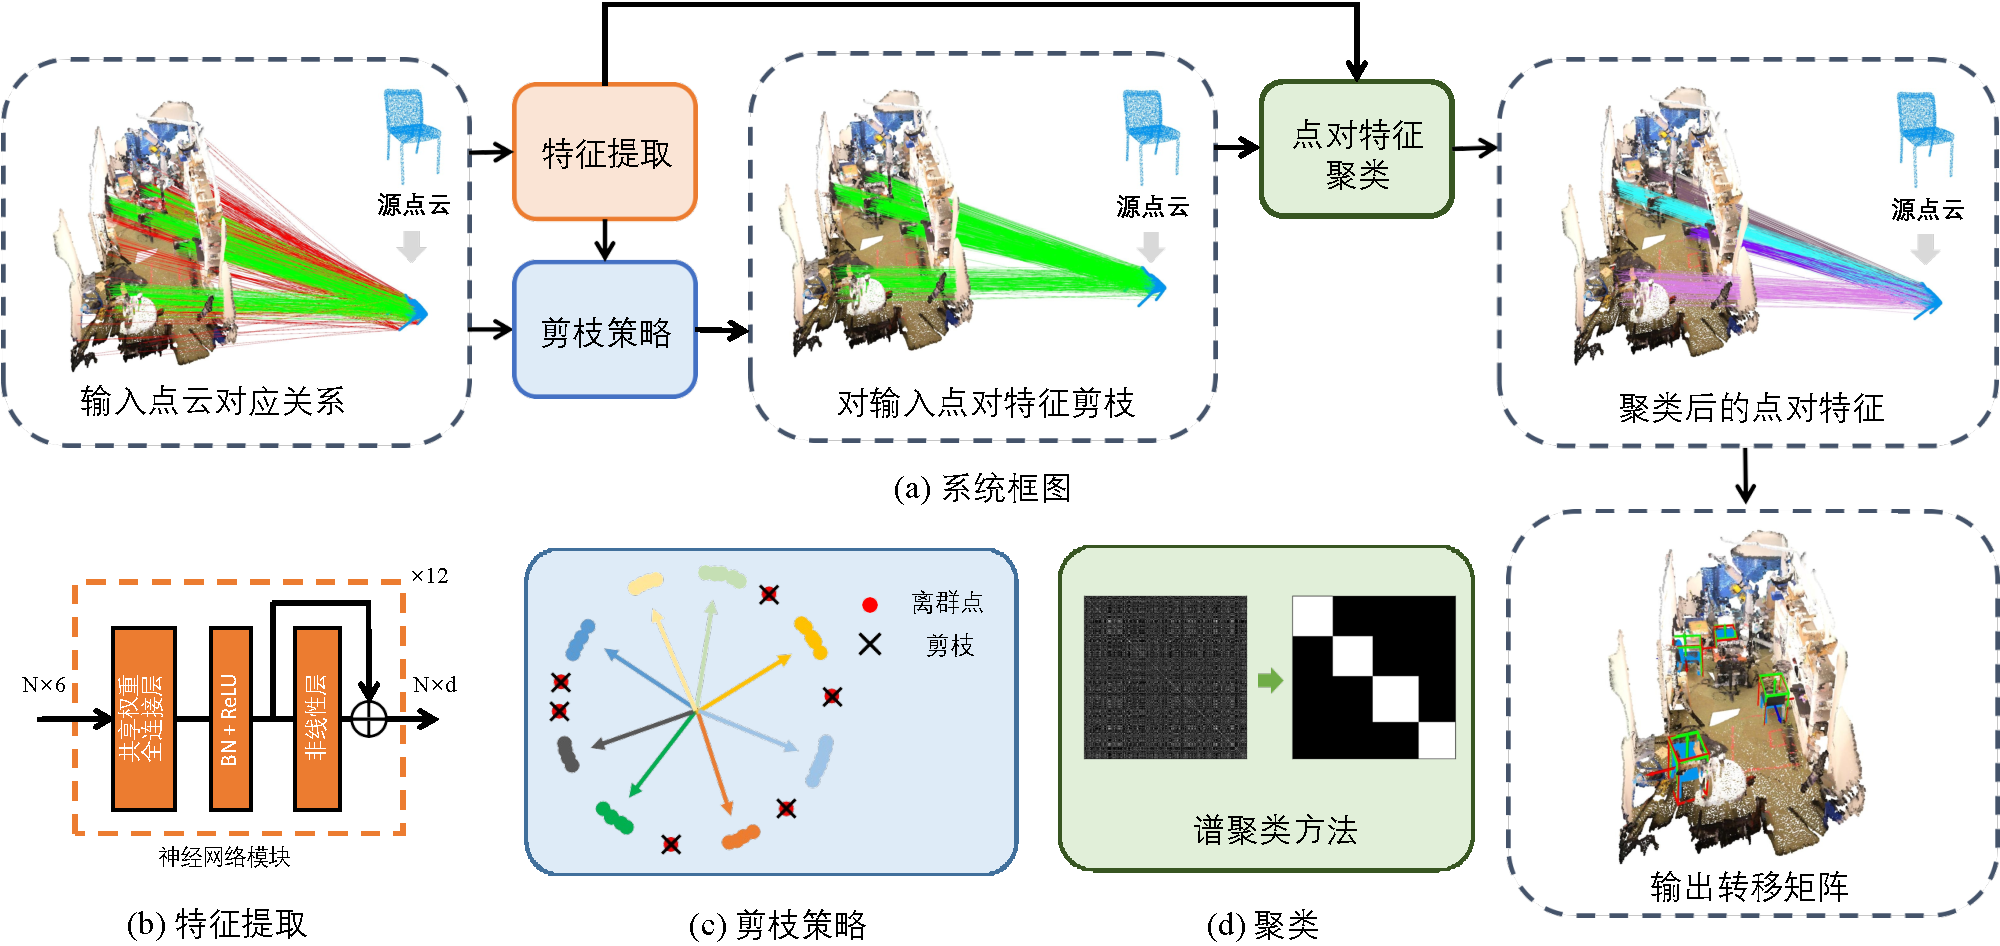
\includegraphics[width=1.0\textwidth]{images/pointcorr.pdf}
    \caption{
        基于深度学习的多实例点云配准框架的流程。     
    }
    \label{fig:point-pipeline}
    \vspace{-0.5in}
  \end{figure}

\subsection{系统模型}
在这一部分中,本文将展示本文的多实例点云配准框架,如图 \ref{fig:point-pipeline} 所示。
本文的框架接受特征匹配生成的假定点对关系作为输入,并首先利用通过对比学习训练的特征提取器来为输入的点对关系提取深度表征(节 \ref{sec:feature_extr})。
然后,本文根据空间一致性和它们的深度表征的相似性来剪枝点对关系(节 \ref{sec:pruning})。
最后,本文聚类剩余的点对关系,并使用聚类结果估计多个实例的变换(节 \ref{sec:clusterandtransform})。

\subsection{特征提取器}\label{sec:feature_extr}
本文框架的第一阶段将 $N$ 个输入的假设点对关系 $C=\left\{c_{i}\right\}_{i=1}^{N}$ 嵌入到特征空间中,以获取均匀分布的 $d$ 维表征 $F=\left\{f_{i} \in \mathbb{R}^{d}\right\}_{i=1}^{N}$,用于后续的剪枝和聚类。
这里,本文采用了 \cite{bai2021pointdsc} 中的 SCNonlocal 模块作为本文的特征提取器,它由 12 个重复块组成。
如图 \ref{fig:point-pipeline}(b) 所示,每个块由一个共享的感知器层、一个带有 ReLU 的 BatchNorm 层和一个 nonlocal 层组成。nonlocal 层整合了刚性变换的空间一致性 \cite{leordeanu2005spectral} 。
在计算每层的特征之前,首先计算一个空间一致性矩阵 $\beta$:
\begin{equation}
  \beta_{i j}=\left[1-\frac{d_{i j}^{2}}{\sigma_{d}^{2}}\right]_{+}, d_{i j}=\left|\left\|x_{i}-x_{j}\right\|-\left\|y_{i}-y_{j}\right\|\right|
\end{equation}
其中,$\sigma_{d}$ 是一个距离参数,用于控制对长度差异的敏感度,$[.]_+$ 表示一个夹紧函数 $max(x,0)$ 以使得 $\beta_{ij} \geq 0$。
nonlocal 层使用 $\beta$ 聚合中间特征:
\begin{equation}
  f_{i}^{k+1}=f_{i}^{k}+M L P\left(\sum_{j=1}^{|C|} \operatorname{soft} \max _{j}(\alpha \beta) g\left(f_{j}^{k}\right)\right)
\end{equation}
其中,$\alpha$ 表示第 $k$ 块中的中间特征表征 $f_i^k$ 和 $f_j^k$ 之间的嵌入点积相似度,$g(\cdot)$ 表示一个线性投影函数。关于网络的更多细节可以在 \cite{bai2021pointdsc} 中找到。

本文利用对比学习来训练本文的特征提取器,以获取均匀分布的深度表征 $F=\left\{f_{i} \in \mathbb{R}^{d}\right\}_{i=1}^{N}$。具体来说,对于一个锚定点对关系 $c_{m i} \in C_{m}^{g t}$,本文将 $C_m^{gt}$ 中的其他点对关系定义为其正样本,并将 $C \backslash C_{m}^{g t}$ 中的点对关系定义为其负样本。本文将特征空间中到锚定点对关系欧几里得距离最小的负样本定义为最难的负样本。在每次迭代中,本文穷尽所有内点作为锚点,并选择他们最难的负样本来构建最难负样本集合 $\mathcal{N}$,并随机选择正样本来构建正样本集合 $\mathcal{P}$。本文的对比损失被定义为:
\begin{equation}
  \mathcal{L}=\sum_{(i, j) \in \mathcal{P}}\left[D\left(f_{i}, f_{j}\right)-m_{p}\right]_{+}^{2} /|\mathcal{P}|+\sum_{(i, j) \in \mathcal{N}}\left[m_{n}-D\left(f_{i}, f_{j}\right)\right]_{+}^{2} /|\mathcal{N}|
  \label{loss}
\end{equation}
其中 $m_p$ 和 $m_n$ 是正样本和负样本的距离阈值,它们防止网络过拟合 \cite{lin2015Deephash}。由于输入点对关系的内点率通常不高,本文可以将输入点对关系下采样到合适的规模,本文对所有负样本的穷举,以找到每个小批量的最难样本是可行的。本文的消融实验显示,利用最难的负样本在提出的方法的高性能中起着重要的作用。

通过优化等式 \ref{loss} 中的损失,属于不同实例的点对关系的表征在特征空间中易于分离,而属于同一实例的点对关系的表征聚集在一起。然后,本文使用这些均匀分布的表征进行剪枝和聚类。本文的实验表明,深度表征提供了空间一致性没有的信息,这使得剪枝和聚类更加有效。

\subsection{剪枝策略}\label{sec:pruning}
输入的点对关系往往包含大量的异常值,这严重破坏了后续的内点点对关系聚类和变换估计。因此,一种直观的想法是首先剪枝输入的点对关系以去除异常值。过去已经提出了一系列的剪枝策略。例如,可以基于相似性阈值 \cite{heckel2013subspace} 或置信度 \cite{zhao2021progressive} 对输入进行剪枝。在本文中,本文提出了一种基于密度的剪枝策略,它根据在第 \ref{sec:feature_extr} 节中学习到的深度表征以及空间一致性约束对输入点对关系进行剪枝。

如第 \ref{sec:feature_extr} 节所述,通过对比学习,满足相同刚性变换的点对关系在特征空间中有相似的表征,且它们远离其他点对关系。这意味着在内点周围的特征密度高于在异常值周围的特征密度 \cite{torr2002napsac} 。基于这个想法,本文设计了一个基于密度的剪枝策略,如图 \ref{fig:point-pipeline}(c) 所示。本文将红色的孤立点视为异常值并移除,而保留其他颜色的聚类点。本文的剪枝方法的详细步骤如下。

本文首先使用提取的深度表征 $F=\left\{f_{i} \in \mathbb{R}^{d}\right\}_{i=1}^{N}$ 来计算点对关系之间的特征相似性矩阵 $S^F$:
\begin{equation}
  S_{i j}^{F}= \, <f_{i}, f_{j}>
\end{equation}
其中 $<\cdot>$ 表示点积。然后,本文使用特征相似性矩阵 $S^F$ 和空间一致性矩阵 $\beta$ 来计算相似性矩阵 $S$:
\begin{equation}
  S=S^{F} \otimes \beta
\end{equation}
其中 $\otimes$ 表示元素乘积,空间一致性矩阵 $\beta$ 在之前已经计算过了。

其次,本文设置一个阈值 $\tau_{S}$ 并用它来将相似性矩阵 $S$ 二值化为二进制相似性矩阵 $\hat{S}$。当第 $i$ 个点对关系和第 $j$ 个点对关系同时在特征空间中满足足够的空间一致性和相似性时,$\hat{S}_{ij}=1$,否则 $\hat{S}_{i j}=0$。现在,本文可以将输入点对关系视为图的节点,$\hat{S}$ 视为图的邻接矩阵。内点集可以被视为具有一定规模的子图,而异常值则出现为孤立点或小规模子图。

最后,本文对二进制相似性矩阵 $\hat{S}$ 的行进行求和,并选择行和值大于阈值 $\tau_N$ 的点对关系。如图 \ref{fig:point-pipeline} (a) 所示,本文的剪枝方法可以有效地去除大部分甚至所有的异常值。本文的实验也证明了剪枝步骤对本文的方法的重要性。本文还在补充材料中提供了如何选择阈值 $\tau_S$ 和 $\tau_N$ 以及消融实验的详细信息。

\subsection{聚类和变换估计}\label{sec:clusterandtransform}
经过剪枝后,本文得到了一个干净的点对关系集合,这个集合几乎没有异常值。下一步是将这些点对关系划分为属于不同实例的多个子集,并估计所有实例的最终刚性变换。点对关系的划分可以被视为一个聚类问题,实例的数量应该等于聚类的数量。在这里,本文使用了一种能够自动确定聚类数量的谱聚类算法 \cite{von2007tutorial,li2007noise}。该算法包括以下步骤:

步骤1:使用剩余点对关系的特征相似性和空间一致性重新计算二进制相似性矩阵 $\hat{S}_n$,其中 $n$ 表示剪枝后的点对关系数量;

步骤2:计算矩阵 $\hat{S}_n$ 的标准化拉普拉斯矩阵 $\hat{L}_n$,并计算标准化拉普拉斯矩阵的特征值 $\lambda_{1}\left(\hat{L}_{n}\right) \leq \lambda_{2}\left(\hat{L}_{n}\right) \leq \ldots \leq \lambda_{n}\left(\hat{L}_{n}\right)$;

步骤3:通过以下公式确定聚类数量 $M$:
\begin{equation}
  \label{eq:cluster}
  M=\underset{k}{\arg \max }\left\{\lambda_{k+1}\left(\hat{L}_{n}\right)-\lambda_{k}\left(\hat{L}_{n}\right)\right\}
\end{equation}

步骤4:应用具有 $M$ 个聚类的谱聚类 \cite{von2007tutorial} 。

由于深度表征在特征空间中有良好的分布,二进制相似性矩阵 $\hat{S}_n$ 符合 \cite{li2007noise} 中定义的理想矩阵。因此,由公式 \ref{eq:cluster} 确定的聚类数量是可靠的,这在 \cite{li2007noise} 中得到了证明。

在以上步骤之后,剩余的点对关系被分配到不同的聚类中,如图 \ref{fig:point-pipeline}(a) 所示,然后本文可以使用如 RANSAC \cite{fischler1981random} 等求解器来估计每个实例的刚性变换。因为本文的剪枝和聚类策略非常有效,每个实例的内点率很高,只需要几十次 RANSAC 迭代就能达到出色的性能。

\subsection{训练细节}
本文在 Pytorch 中实现了本文的网络,并使用 scikit-learn \cite{Pedregosa2011Scikit} 实现谱聚类。
本文随机地将输入点对关系下采样到1000。
对于合成数据集,距离参数 $\sigma_d$ 被设置为 0.05,对于真实数据集,被设置为 0.1。
本文将深度表征的维数 $d$ 设置为 128。
阈值 $\tau_S$ 被设置为 0.85。
对于合成数据集,阈值 $\tau_N$ 设置为 10,对于真实数据集,设置为 20。
边缘 $m_p$ 和 $m_n$ 分别设置为 0.1 和 1.4。
本文的批量大小设置为 16。
本文使用 ADAM 优化器优化网络,初始学习率为 0.01,并训练网络 15K 次迭代。
所有实验都在 NVIDIA GPU 3090Ti 图形卡上进行。

\section{小结}
本章,本文介绍了提出的两种多实例点云配准流程,高效对应聚类的多实例点云配准和基于深度学习的多实例点云配准,这两种方法均需要通过好的方法来得到好的点云点对关系。下面本文将对这两种方法进行实验验证。